\documentclass{beamer}
\usetheme{Intel}

%\setbeameroption{show notes} % If annotations are desired.
\setbeamertemplate{section in toc}{\inserttocsectionnumber.~\inserttocsection} % Use number keys for table of content sections.
\setbeamertemplate{subsection in toc}{\hspace{0.5cm}\rule[0.3ex]{3pt}{3pt}~\inserttocsubsection\par} % Use a symbol for table of content subsections.
\AtBeginSection[]
{
	\begin{frame}
		\frametitle{Table of Contents}
		\begin{multicols}{2}
			\tableofcontents[currentsection]
		\end{multicols}
    \end{frame}
} % Insert table of contents frame before each new section.
\setbeamertemplate{caption}[numbered] % Number figures.

\definecolor{intel}{RGB}{0, 113, 197}
\setbeamercolor{section in toc shaded}{fg=intel}
\setbeamercolor{subsection in toc shaded}{fg=black}
\setbeamercolor{section in toc}{fg=intel}
\setbeamercolor{subsection in toc}{fg=black}
\setbeamercolor{block title}{fg=intel}
\setbeamercolor{caption name}{fg=intel}

\usepackage{hyperref} % Used to invoke Santa Claus.
\usepackage{multicol} % Used to split up table of contents in a double column style.
\usepackage{multirow} % Needed for multirow graphs
\usepackage{datetime} % Used to format dates.
\usepackage{listings} % Used to format inline code throughout document.
\usepackage{color} % Used to gray out text
\usepackage{tikz} % Used to gain access to the \centering command.
\usepackage[mediumspace,mediumqspace,squaren,binary]{SIunits} % \milli\second

\usepackage[footinfo]{gitinfo} % dv2524-pac/

\hypersetup{
	colorlinks=false,
	linkcolor=blue,
	urlcolor=black,
	citecolor=blue,
	anchorcolor=blue
}
\usetikzlibrary{calc}

\newenvironment{graytext}{\color{gray}}{\ignorespacesafterend}

\newcommand{\mascfirstline}[1]{\input{#1}\unskip}

\lstset{
	language=C,
	tabsize=4,
	backgroundcolor=\color{black!5},
	basicstyle=\tiny,
}

% Formatting inline code command:
\newcommand{\dvtcmdcodeinline}[1]{
	\colorbox{black!5}{
			\lstinline[basicstyle=\ttfamily\color{black}]{#1}}}

\newtheorem{thm}{Key point}

\begin{document}
	% FRONT MATTER
	% ---
	\title{Paravirtualizing OpenGL ES in Simics}
\subtitle{Master's Thesis in Computer Science}
\author{Eric Nilsson}
\institute{Intel Corporation}
\date{\today}

\begin{frame}
	\titlepage
\end{frame}


	% BODY MATTER
	% ---
	% INTRODUCTION
	\section{Introduction}
	% Simics
	\subsection{Simics}
	\input{simics.tex}
	% Graphics virtualization
	\subsection{Graphics virtualization}
	\input{graphicsvirtualization.tex}
	% Summary
	\subsection{Summary}
	\begin{frame}
  \frametitle{Summary}

  \begin{block}{Method}
    \begin{itemize}
    \item Paravirtualized graphics in Simics
    \item Accelerates OpenGL ES 2.0
    \end{itemize}
  \end{block}

  \begin{block}{Evaluation}
    \begin{itemize}
    \item Run benchmarks stressing suspected optimal and sub-optimal use-case
    \item Compare performance to software rasterization
    \end{itemize}
  \end{block}

  \begin{block}{Conclusion}
    \begin{itemize}
    \item Performance improvements (up to $34$ times)
    \item Located bottleneck
    \end{itemize}
  \end{block}

\end{frame}

	% Key points
	\subsection{Key points}
	\begin{frame}
\frametitle{Key points}

\begin{block}{\#1}
	Paravirtualization is a viable method of accelerating graphics
\end{block}

\begin{block}{\#2}
	Magic instructions is a suitable communications medium
\end{block}

\begin{block}{\#3}
	The case for paravirtualization is strengthened for systems where hardware-assisted virtualization is unavailable
\end{block}

\end{frame}


	% PARAVIRTUALIZATION
	\section{Methodology}
	% Overview
	\subsection{Overview}
	\input{overview.tex}
	% Magic instructions
	\subsection{Magic instructions}
	\input{magicinstructions.tex}
	% Simics Pipe
	\subsection{Simics Pipe}
	\begin{frame}
\frametitle{Simics Pipe}

\begin{center}
	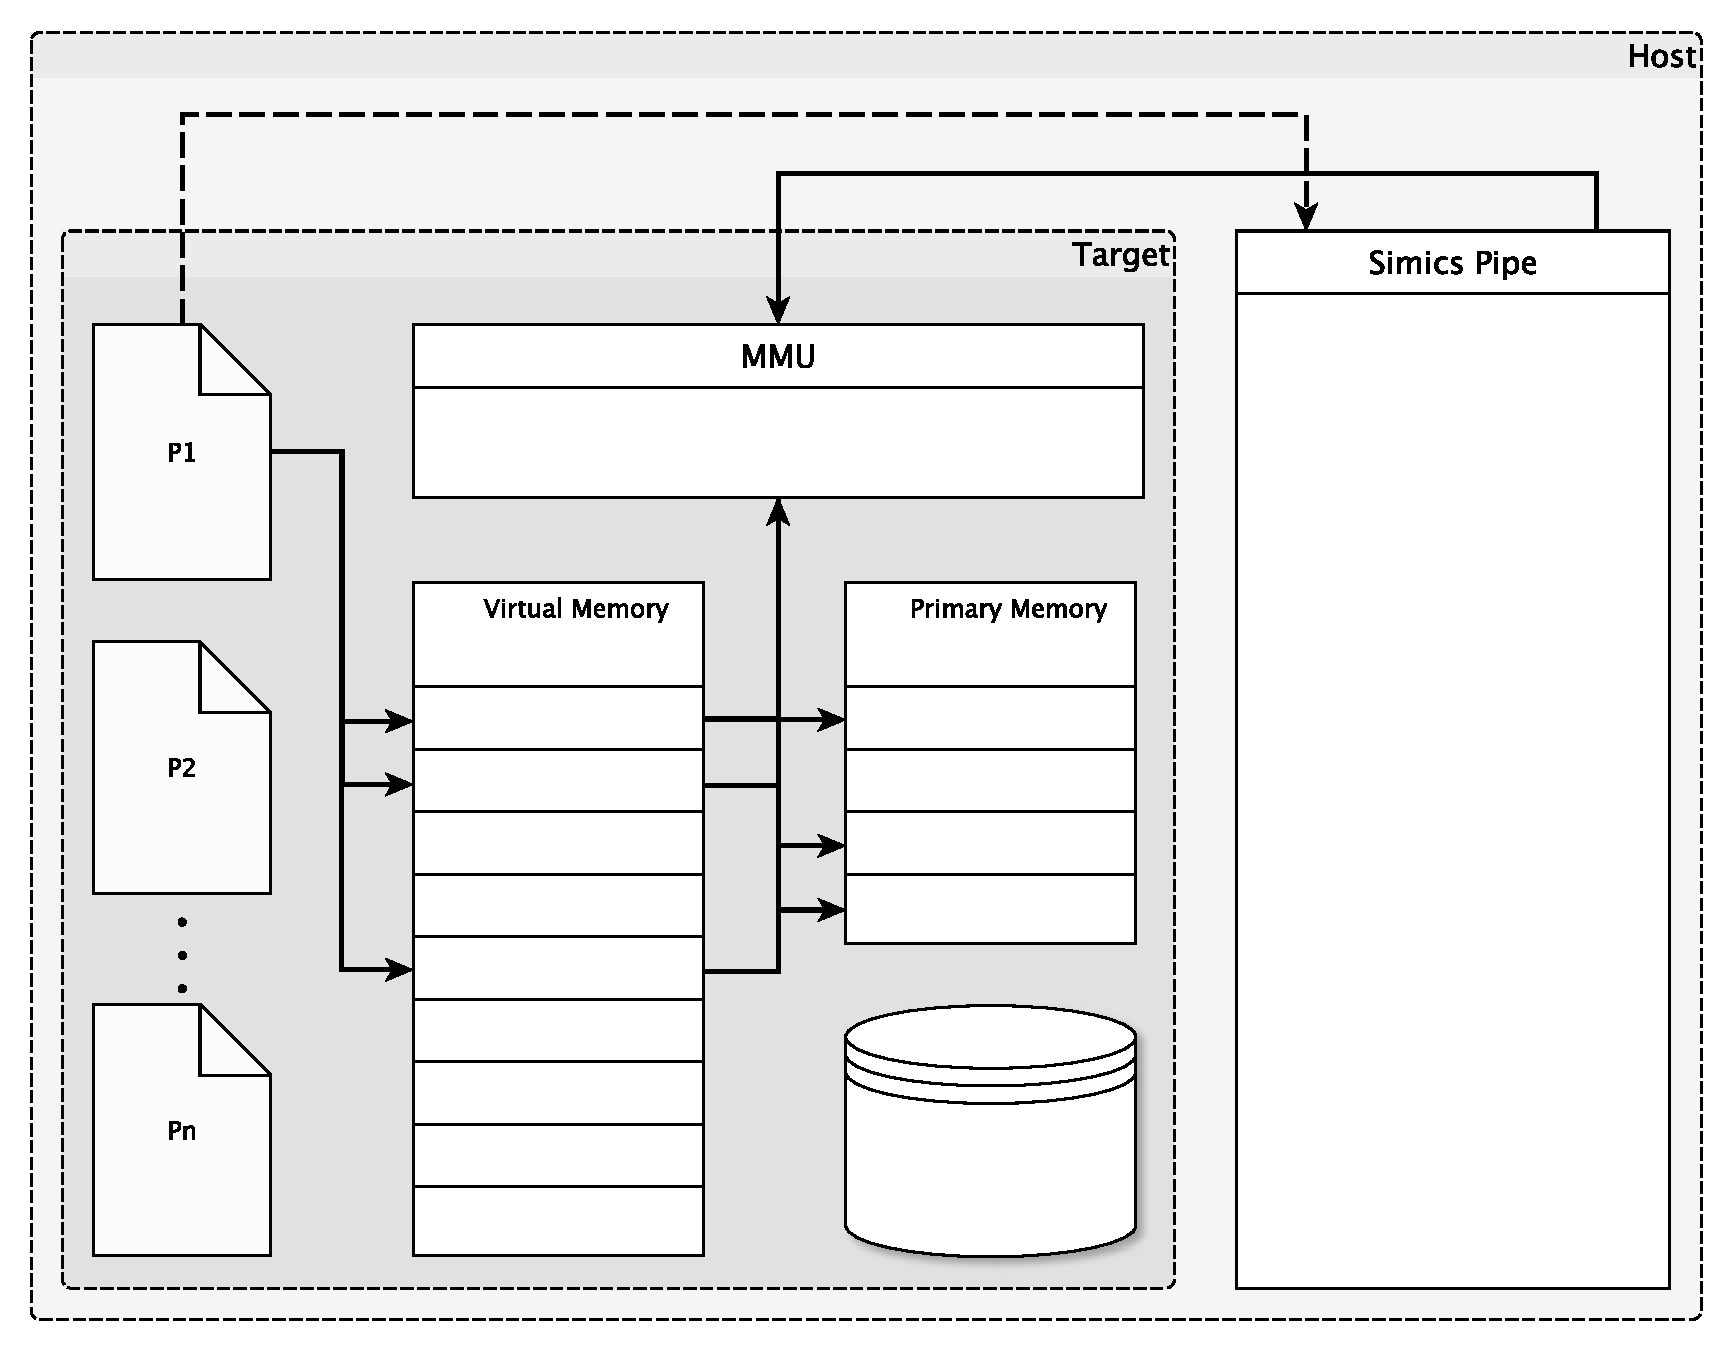
\includegraphics[height=0.8\textheight]{yedvirtualmemory.pdf}
\end{center}

\end{frame}

%% Memory translation overview. The OpenGL process hands a virtual memory
%% address, pointing somewhere in the target system \textit{primary}
%% memory, to the paravirtualized solution - which inquiries the target
%% system MMU to retrieve designated bytestream directly from target
%% physical memory.


	% EXPERIMENT
	\section{Experiment}
	% Benchmarks
	\subsection{Benchmarks}
	\begin{frame}
\frametitle{Benchmarks}

\begin{columns}
  \column{0.5\textwidth}

  \begin{block}{Chess}
    \begin{itemize}
    \item Many lightweight draw calls
    \item Induces many magic instructions, stresses communication latency
    \end{itemize}
  \end{block}

  \begin{block}{Julia}
    \begin{itemize}
    \item Heavy-duty shader
    \item Renders Julia fractal
    \end{itemize}
  \end{block}

  $10$ to $20$ ms per frame on host; $16$ ms frame time $\approx60$ FPS
  
  \column{0.5\textwidth}

  \includegraphics[width=0.45\linewidth]{imgchess.png}
  \hspace{0.2cm}
  \includegraphics[width=0.45\linewidth]{imgjulia.png}

\end{columns}
	
\end{frame}


	% RESULTS
	\section{Results}
        \input{tables.tex}
	\subsection{Histograms}
	\input{resultshistograms.tex}
	% Magic instruction overhead
	\subsection{Magic instruction overhead}
	\input{magicinstructionoverhead.tex}

	% DISCUSSION
	\section{Discussion}
	% Deterministic execution
	\subsection{Deterministic execution}
	\input{deterministicexecution.tex}
	% Checkpointing
	\subsection{Checkpointing}
	\input{checkpointing.tex}
	% Reverse execution
	\subsection{Reverse execution}
	\input{reverseexecution.tex}

	% CONCLUSION
	\section{Conclusion}
	% Demonstration
	\subsection{Demonstration}
	\input{demonstration.tex}
	% Future work
	\subsection{Future work}
	\begin{frame}

\frametitle{Future work}

\begin{itemize}
  \item Command serialization batching \begin{itemize}\item WireGL\end{itemize}
  \item Extending supported frameworks \begin{itemize}\item DirectX $\rightarrow$ OpenGL\end{itemize}
  \item General purpose, GPGPU \begin{itemize}\item OpenCL\end{itemize}
\end{itemize}

\end{frame}

	% Key point recap
	\subsection{Key points recap}
	\begin{frame}
\frametitle{Key points}

\begin{block}{\#1}
	Paravirtualization is a viable method of accelerating graphics
\end{block}

\begin{block}{\#2}
	Magic instructions is a suitable communications medium
\end{block}

\begin{block}{\#3}
	The case for paravirtualization is strengthened for systems where hardware-assisted virtualization is unavailable
\end{block}

\end{frame}

\end{document}
